\documentclass[12pt]{article}
\usepackage{graphicx}
\usepackage{subcaption}
\usepackage{hyperref}
\usepackage{float}
\usepackage{mathtools}

\title{CMSC 6950 Project}
\date{June 2021}
\author{Kabir Zubaer} 

\setlength\parindent{0pt}
\begin{document}
\maketitle
\section{Introduction}

Water covers more than two-thirds of the Earth’s surface. The deep waters are home to wildlife and some of the enormous creatures on Earth. Argo brings a solution for oceanographers to monitor the Global Ocean. It is a worldwide network of almost 4000 independent probes measuring pressure, temperature, and salinity from the surface to 2000m depth every ten days. The probes installed in every 60o parallels and information from the ocean are collected using satellite. The authority managed several data centers, merged in a single dataset which is open for all. The dataset is available using ftp server or monthly zip snapshots.

Argo dataset is complex to understand and difficult to access Argo data consists of thousands of files. In this project I used A Python library for Argo ocean data analysis called Argopy. Argopy has two critical features made it easier for the users, these are its Data fetching and its ability to provide data formatting. In this project, I have included both Data fetching and data formatting features. 

\section{Results}

Herein, the results for each computational task will be presented. The first computational task will focus on visualizing the position of Argo floats in a region Oceania,  and how the total number of floats changes each year. The second computational task is used to visualize the trajectory and temperature variation of two Argo floats with time since the float's deployment.
  
\subsection{Task 1- Total Argo float numbers through time}
The aim of my first computational task is to retrieve Argo float data collected from June 2015 to December 2015 using argopy and then use this data to visualize the change in the total number of Argo floats per month within a region of the Oceania.  



\verb|Data fetching|

One of the features of Argopy is import data using the API of Argo data through a simple call. To fetch data from argo I used following tecnique:
\begin{itemize}
     \item import data using  \verb|DataFetcher as ArgoDataFetcher|
     \item Fetch data between 140/150W, 35/, 50N, from 0 to 100db and from June 2015 to December 2015
    \item Next use \verb|argo_loader.region().to_xarray()| which takes longitude, latitude, and time period as arguments, and 
     returns the argo data in multidimensional \verb|xarray|.
     \item Finally .
\end{itemize}
Change in  for an area of interest within a certain time frame.


The image explains the total number of Argo floats data of the Oceania collected from June 2015 to December 2015.

\begin{figure}[H]
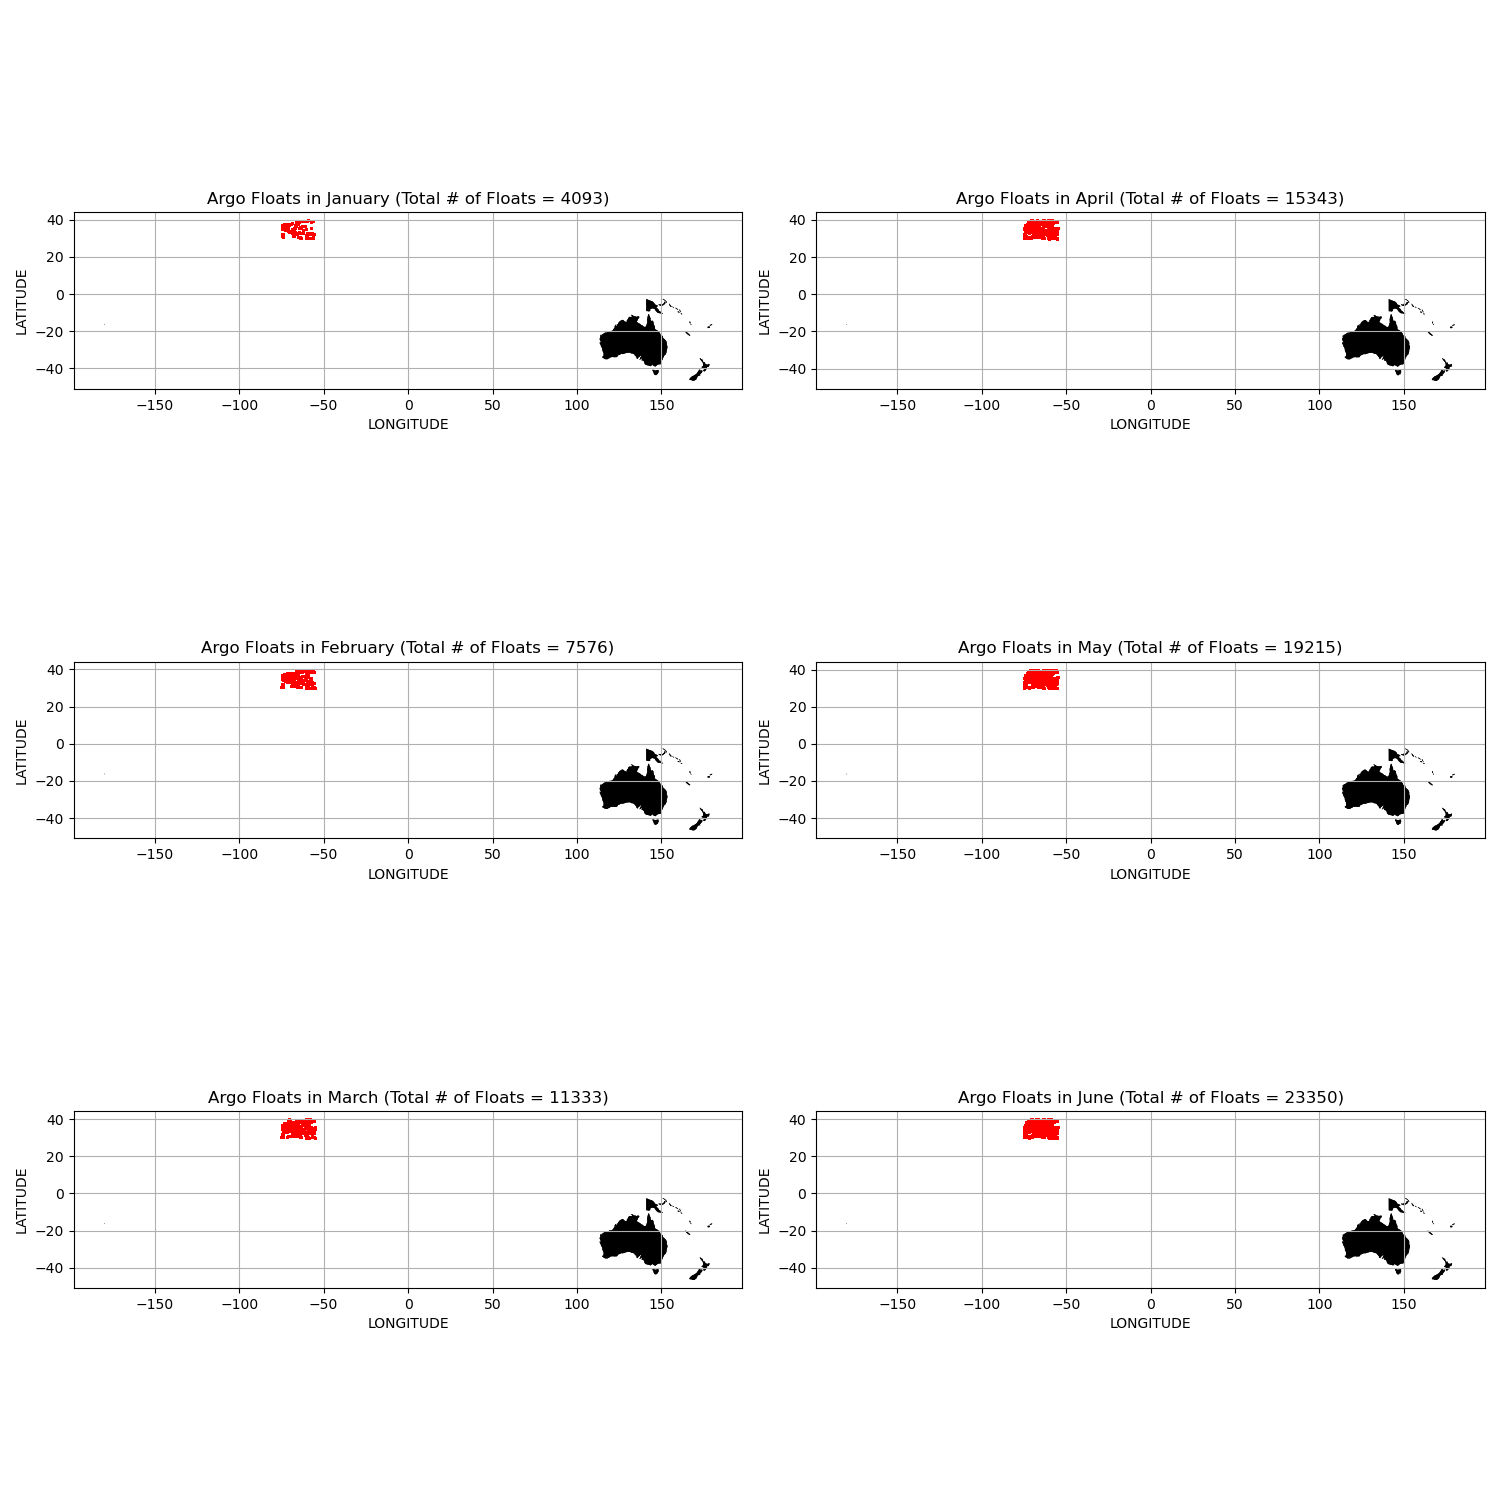
\includegraphics[width=\textwidth,height=\textheight,keepaspectratio]{monthly.png}
\caption{Total number of Argo floats for each month from June 2015 to December 2015  in a region Oceania.}
\label{fig:task 1}
 
\end{figure}

\subsection{Task 2 - Showing Level, Pressure, Salinity, and Temperature through time.}

In this task I try to find out Level, Pressure, Salinity, and Temperature for each month from June 2015 to December 2015  in a region Oceania

\begin{figure}[H]
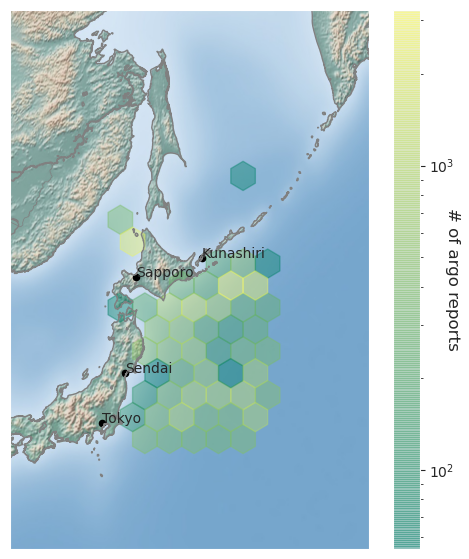
\includegraphics[width=\textwidth,height=\textheight,keepaspectratio]{locations.png}
\caption{Hexbin of Argo floats for each month from June 2015 to December 2015  in a region Oceania.}
\label{fig:task 2}
 
\end{figure}

\section{Conclusion}
In this task, I try to solve two computational tasks involving argopy, I have fetched data from external sources for the period of six months. In case of ploting and visualization I used different python library.


\begin{thebibliography}{9}
    \bibitem{latexcompanion} 
    Maze et al.,
    \textit{argopy: A Python library for Argo ocean data analysis.}. 
    Journal of Open Source Software, 5(53), 2425, 2020.
\end{thebibliography}

\end{document}
